\clearpage
\section{Model Verification}
\label{sec:modelVerification}

In order to test our model, a set of verification data \textbf{disjoint} from the training data are used. Three different sets of power values is used to test the model against the following performance indices:

\begin{itemize}
	\item Integral squared error (ISE) = $\sum _{t=0}^{N}(y _{model}(t) - y _{est}(t))^2$ 
    \item Integral absolute error (IAE) = $\sum _{t=0}^{N}|y _{model}(t) - y _{est}(t)|$ 
    \item Integral time squared error (ITSE) = $\sum _{t=0}^{N}t(y _{model}(t) - y _{est}(t))^2$ 
    \item Integral time absolute error (ITAE) = $\sum _{t=0}^{N}t|y _{model}(t) - y _{est}(t)|$ 
\end{itemize}
Where $y _{est}$ is the signal used to in verification 
and $y _{model}$ is the signal generated by our model

The output, $y _{model}$ is generated using the estimated model parameters. Its time response is given by:

\begin{equation}
y _{model}(t) = [q + 2N\me^{-\xi \omega _nt}\cos (\omega _n\sqrt{1 - \xi^2t} + \phi)]\textbf{1}(t)
\end{equation}
With $N = \frac{q}{2\sqrt{1-\xi^2}}$ and $\phi = \arctan (\frac{\xi}{-\sqrt{1-xi^2}})$.
\newline
$q$ is the final value of $y _{est}(t)$ and is given by:

\begin{equation}
	\lim _{t\to +\infty}y _{est}(t) = q
\end{equation}
Which is the estimated steady state value of $y _{est}(t)$.

The table below summarizes performance indices for the 3 sets of verification data used.

\begin{tabular}{| l | l | l | l | l |}
\hline
 Power & ISE & IAE & ITSE & ITAE \\
 \hline
30 & 81089.78& 21302.75& 1203.23& 1458.55 \\
\hline
80 & 42799.34&12731.58 &4023.19 & 6826.76 \\
\hline
100 & 54420.04& 13518.735& 3664.89& 678.25  \\
\hline
\end{tabular}

\begin{figure}[H]
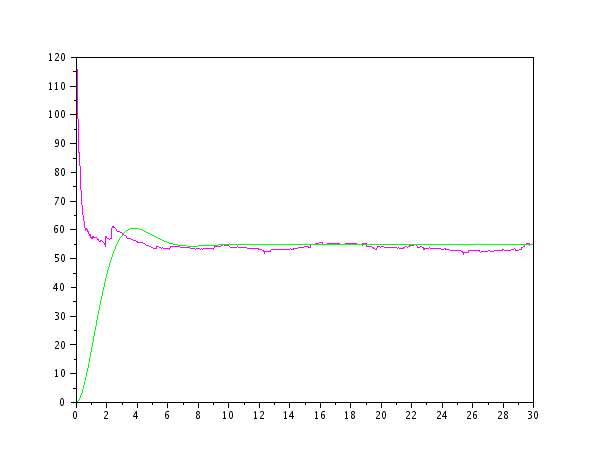
\includegraphics[scale=0.5]{images/100_dat_performance.png}
\caption{A graph showing the signals $y _{model}(green)$ and $y _{est}$ for the power value=100}
\end{figure}

